\documentclass[12pt]{article}

\usepackage{stylefile}

\begin{document}

\Exlabelsep = 0.2\parindent
\SubExleftmargin = 1.2\parindent

\begin{center}
\noindent\LARGE \textbf{Exclusive disjunction} \\[.5cm]
\large Michael Franke\\[.1cm] 
\large Bob van Tiel
\end{center}

\begin{abstract}
If someone says `Donald ate a pretzel or a donut' the hearer may infer that Donald did not eat both a pretzel and a donut. This exclusive reading of `or' is often explained as a scalar implicature. We tested this explanation by investigating how the robustness of the exclusive reading of `or' is influenced by three contextual factors: relevance, competence, and prior probability. We found that only prior probability has a significant effect on the robustness of the exclusive reading, thus disconfirming the scalar implicature account. Instead, we propose that the exclusive reading of `or' is a probabilistic inference based on world knowledge.
\end{abstract}

%--------------------------------------------------------
\section{Introduction}
%--------------------------------------------------------

Introductions to logic usually distinguish between two readings of `or': an inclusive and an exclusive reading \citep[e.g.,][]{mccawley1981, copi2005}. The inclusive reading corresponds to the meaning of logical disjunction. According to this reading, `$A$ or $B$' is true if at least one and possibly both of $A$ and $B$ are true. The exclusive reading is more strict in that it excludes the possibility that both $A$ and $B$ are true. So on its exclusive reading, `$A$ or $B$' is true if exactly one of $A$ and $B$ is true. To illustrate, consider:

\ex.	\label{ex:support} Joe supports Donald or Hillary.

On its inclusive reading, this sentence is true whenever Joe supports Donald, Hillary, or both. The exclusive reading, which is arguably more prominent in this example, excludes the latter possibility. That is, on its exclusive reading, \Last is true whenever Joe supports Donald or Hillary, but not both.

The presence of these two readings might suggest that `or' is associated with two different lexical entries \citep[e.g.,][]{basson1960, baum1996, rescher1964}. There are, however, good reasons to reject such a lexicalist approach. Perhaps the most compelling reason is that, in some contexts, `or' can only receive one interpretation. To illustrate, consider the following sentence, in which `or' occurs in the scope of negation:

\ex.	 Joe does not support Donald or Hillary.

This sentence has only one interpretation, namely that Joe supports neither Donald nor Hillary \citep[cf.][]{crain2008}. This interpretation corresponds to the inclusive reading of `or'. It does not have an interpretation corresponding to the exclusive reading; in other words, it does not have a reading according to which Joe either supports both Donald and Hillary, or neither of them. Since `or' is systematically monosemous in certain contexts---negation being one of them---it follows that the two readings of `or' cannot simply be due to a lexical ambiguity.

An attractive alternative to the lexicalist approach stems from Grice's \citeyearpar{grice1975} theory of conversational implicature. According to Grice, natural conversation is governed by the assumption that speakers are cooperative; that is, they attempt to further the purpose of the discourse by means of their utterances. Speakers are cooperative by adhering to four maxims that enjoin their utterances to be truthful, informative, relevant, and clear. Sometimes hearers have to make ancillary assumptions in order to align a speaker's utterance with the assumption of cooperativity. Such ancillary assumptions are called \emph{conversational implicatures}. An example, from Grice's own work, is given in the following conversation:

\ex.	A: I am out of petrol. \\
 B: There is a garage around the corner.
	
B's utterance would be irrelevant, and hence uncooperative, if he knew that the garage was closed or did not sell petrol. Since A assumes that her interlocutor is cooperative, she thus concludes that the garage is open and sells petrol.

\citet{horn1972} was the first to argue that the exclusive reading of `or' can be explained as
a conversational implicature, too, based on the assumption that the primary meaning of `or' is
inclusive. To illustrate, consider \ref{ex:support} again. Assuming that the primary meaning of
`or' is inclusive, the speaker of \ref{ex:support} could have been more informative, and hence
cooperative, by saying `Joe supports Donald and Hillary.' Why didn't she? Presumably because
she does not believe that this alternative is true. This is a weak inference that is compatible
with a situation in which the speaker is unsure about whether or not Joe supports both Donald
and Hillary. This weak inference can be strengthened if there is reason to believe that the speaker knows whether or not Joe supports both Donald and Hillary. This assumption is often called the \emph{competence assumption}. If the competence assumption is sufficiently plausible, it follows that, according to the speaker, Joe does not support both Donald and Hillary.

This specific kind of conversational implicature is often called a \emph{scalar implicature} because it is assumed that `or' forms a lexical scale with `and', and that alternatives are generated by substituting the scalemates `or' and `and'. Other lexical scales are $\langle$some, all$\rangle$, $\langle$warm, hot$\rangle$, and $\langle$intelligent, brilliant$\rangle$ \citep[cf. e.g.,][]{tiel2016}.

The implicature account straightforwardly explains the absence of exclusive readings under negation. Consider \LLast again. Here, unlike in the case of \ref{ex:support}, the alternative with `and' is less informative than the utterance itself. After all, \LLast is only compatible with a situation in which Joe supports neither Donald nor Hillary, whereas the sentence with `and' is also consistent with situations in which Joe supports exactly one of Donald and Hillary. So the speaker was already maximally informative and hence no implicature is derived.

Although the implicature account has since become the standard in the literature \citep[e.g.,][]{chevallier2008, chierchia2012, fox2007, sauerland2004, geurts2010}, it is not without its problems, as we will see in the next section. Therefore, we set out to experimentally test the adequacy of the implicature account. To that end, we tested the effect of three factors on the robustness of exclusive readings:\ (i) the \emph{relevance} of the sentence with `and' to the hearer, (ii) the \emph{competence} of the speaker about the truth of the sentence with `and', and (iii) the \emph{prior probability} that the sentence with `and' is true. These factors are usually taken to influence the robustness of scalar implicatures. Hence, if the implicature account is correct, we expect these factors to influence the robustness of the exclusive reading of `or', too. 

For comparison, we also investigated how relevance, competence, and prior probability influence the robustness of a bona fide scalar implicature, namely the inference from `some' to `not all'. To illustrate, consider:

\ex.	Some of my friends support Donald.

An utterance of this sentence may convey that not all of the speaker's friends support Donald. The derivation of this upper-bounding construal runs analogous to that of the exclusive reading of `or': the speaker could have been more informative by saying `All of my friends support Donald'. Why didn't she? Presumably because she does not believe that this alternative is true. If, moreover, the speaker knows whether or not all of her friends support Donald, it follows that she believes not all of her friends support Donald.

As we will see, it turns out that there are marked differences in how relevance, competence, and prior probability influence the robustness of the exclusive reading of `or' compared to how they influence the robustness of the inference from `some' to `not all'. These findings will force us to reconsider the implicature account of the exclusive reading of `or'.

In the next section, we explain our three factors of interest in more detail. Afterwards, we outline the details of our experiments and discuss the results.

%--------------------------------------------------------
\section{Relevance, competence, and prior probability}
%--------------------------------------------------------
%--------------------------------------------------------
\subsection*{Relevance}
%--------------------------------------------------------

Almost all theorists agree that the robustness of scalar implicatures is modulated by various extralinguistic factors (e.g., \citealt{chierchia2012, geurts2010, horn1972, franke2009}, but see \citealt{chierchia2004, levinson2000, storto2005}). Some of these factors are specific to certain theories, while others are shared across competing theories. Relevance is of the latter kind in that it features in almost all theories of scalar inferences. However, relevance is a multivocal notion, and there are at least two construals that should be distinguished:\ relevance for the discourse purpose and relevance for the hearer's interest \citep{geurts2010}.

The notion of relevance for the discourse purpose can be illustrated with the following example (from \citealt{kuppevelt1996}):

\ex.	A: How many of the boys were at the party? \\ B: Some of the boys were at the party.

Discourse purposes are usually equated to questions, which can be implicit or, as in this case, explicit \citep{roberts2012}. A piece of information is relevant if it contributes to answering this question. In \Last, the information that not all of the boys went to the party is relevant to the discourse purpose because it narrows down the space of possible answers. Compare this to a situation in which B's answer addresses the question `Were some of the boys at the party?' In this situation, the upper-bounding construal is irrelevant, since the question is already resolved when `some' is interpreted as `at least some and possibly all'. Hence, it is hypothesised, no scalar implicature will be derived in this situation.

In this paper, however, we will mainly be concerned with the second notion of relevance:\ relevance to the hearer's interest. This construal is intimately connected to \emph{relevance theory} \citep{sperber1995}.

According to relevance theory, the relevance of an inference is determined by two factors: (i) the positive cognitive effects it has on the hearer---i.e., to what extent it makes ``a worthwhile difference to the individual's representation of the world'' \citep[p.\ 251]{wilson2002}---and (ii) the effort needed to process that inference. In what follows, we focus on the first factor, assuming that processing effort remains invariant across the scenarios that we tested (cf.\ \citealt{chevallier2008} for a series of experiments on `or' that manipulate processing effort). 

The central tenet of relevance theory is that communication is aimed at maximising relevance, so that hearers only derive inferences whose positive cognitive effects outweigh their processing cost. Hence, relevance theory predicts that the robustness of a scalar implicature is an increasing function of its importance to the hearer. To illustrate, consider:

\ex.	Donald won the primaries in Nebraska or Indiana.

According to relevance theory, the robustness of the exclusive reading of this sentence depends on how important it is to the hearer whether Donald won the primaries in both Nebraska and Indiana. Suppose, for example, that the hearer made a large bet that Donald would not win both primaries. In that case, she would be more likely to arrive at an exclusive reading than if, for example, she made a large bet that Donald would win at least one of the primaries.

Hence, if relevance theory is correct, we expect the robustness of the inference from `some' to `not all' to be positively affected by the relevance of the upper-bounded reading to the hearer. If, in addition, the implicature account is correct, we expect the same effect on the exclusive reading of `or'.

%--------------------------------------------------------
\subsection*{Competence}
%--------------------------------------------------------

In the previous section, we have seen that competence plays an important role in the derivation of scalar implicatures. Initially, pragmatic reasoning yields a weak inference according to which the speaker does not believe that the more informative alternative is true. This weak inference can be strengthened if the competence assumption holds; that is, if it is assumed that the speaker knows whether or not the more informative statement is true. If so, it follows that, according to the speaker, the more informative statement is false.

Although the workings of the competence assumption tend to be unproblematic for most scalar expressions, they are rather precarious in the case of `or'. Indeed, the need to invoke competence to arrive at an exclusive reading of `or' gives rise to what \citet{zondervan2010} calls the \emph{speaker expertise paradox} \citep[cf.][]{geurts2006}. To explain this paradox, consider \ref{ex:support} once again:

\ex.	Joe supports Donald or Hillary.

We have already seen that someone who utters this sentence implies that Joe does not support
both Donald and Hillary. Presumably, however, the utterance also implies that the speaker does not know whether
Joe supports Donald and that she does not know whether Joe supports Hillary. After all, if the speaker knew that Joe supports Donald, she should have said `Joe supports Donald', and mutatis mutandis if she knew that Joe supports Hillary. However, in order to arrive at the exclusive reading through pragmatic reasoning, it has to be assumed that the
speaker knows whether Joe supports both Donald and Hillary. 

More abstractly, in order to derive
the exclusive reading of a disjunction `$A$ or $B$', it has to be assumed that the speaker is
ignorant about the truth of $A$ and $B$ individually, but knowledgeable about the truth of `$A$ and $B$'. Such an epistemic state is possible but intuitively improbable, which contradicts the observation that exclusive interpretations are far from uncommon.

In order to arrive at a more decisive verdict, however, we tested the effect of competence on the robustness of the exclusive reading of `or' and the upper-bounded construal of `some'. Previous experimental research has shown that the robustness of the upper-bounded reading of `some' increases with the competence of the speaker \citep{goodman2013}. We expect to replicate this effect in our study. If, moreover, the exclusive reading is due to a scalar implicature, we expect a similar effect in the case of `or'.

%--------------------------------------------------------
\subsection*{Prior probability}
%--------------------------------------------------------

Compared to the previous two factors, the role of prior probabilities is more controversial. Some theorists have marginalised the importance of prior probabilities \citep{geurts2010}, while others have assigned them an important role in the derivation of scalar implicatures \citep[e.g.,][]{Russell2012:Probabilistic-R,frank2012, FrankeJager2015:Probabilistic-p}. According to at least some these accounts, the robustness of a scalar implicature is an increasing function of the prior probability that it is true. To
illustrate, consider the following sentence once again:

\ex.	Donald won the primaries in Nebraska or Indiana.

Theories that are sensitive to prior probabilities predict that, if it is deemed extremely unlikely that Donald wins the primaries in both states, someone who hears an utterance of \Last will be more likely to arrive at an exclusive reading of `or', compared to when the hearer is expecting Donald to win both primaries.

Interestingly, a number of theorists have argued that the robustness of exclusive readings is exhaustively determined by prior probabilities \citep[e.g.,][]{rubin1989, yanal1988}. These authors hold that `or' is monosemous and always interpreted inclusively. The appearance of an exclusive reading is caused by probabilistic reasoning about possible states of the world. An especially clear example that illustrates this point is:

\ex.	Joe voted for Donald or Hillary.

Here, it seems that the speaker's utterance rules out the possibility that Joe voted for both Donald and Hillary. According to the aforementioned theorists, this inference is not due to an exclusive reading of `or' but rather to an inclusive reading along with the commonsense information that one can only vote once in a democratic election. In this way, then, world knowledge is responsible for seemingly exclusive interpretations of `or'. Importantly, this position is distinct from the implicature account because it holds that the derivation of exclusive readings does not involve any reasoning about the intentions of the speaker.

Previous experimental research has confirmed that the robustness of the upper-bounded reading of `some' is positively affected by the prior probability that it is true \citep{degen2015}. We expect to replicate that result in our study. In addition, if exclusive readings are due to scalar implicatures, we expect a similar effect in the case of `or'.

%--------------------------------------------------------
\subsection*{Predictions}
%--------------------------------------------------------

In summary, we have discussed three factors that have variously been taken to increase the
robustness of scalar implicatures: (i) the relevance of the more informative statement to the
hearer, (ii) the competence of the speaker about the truth of the more informative statement,
and (iii) the prior probability that the more informative statement is false.

In the next section, we discuss two experiments in which we measured the effect of relevance, competence, and prior probability on the robustness of, on the one hand, the upper-bounded construal of `some' (Exp.\ 1) and, on the other hand, the exclusive reading of `or' (Exp.\ 2). We hypothesise that all three factors influence the robustness of the upper-bounded construal of `some'. More concretely, we hypothesise that the upper-bounding construal of `some' should be  more prominent under higher contextual relevance, higher speaker competence, and lower a priori probability of the corresponding sentence with `all'. If the implicature account is correct, we expect that the exclusive reading of `or' patterns with the upper-bounded construal of `some' in these respects.

Since Exp.\ 1 and 2 share the same methodology, we discuss them in tandem. Afterwards, in Exp.\ 3, we discuss and test an alternative version of the implicature account, according to which statements of the form `$A$ or $B$' are read, in effect, as `$A$ and nothing else or $B$ and nothing else'. 

%--------------------------------------------------------
\section{Experiments 1 and 2}
%--------------------------------------------------------
\subsection*{Design}
%--------------------------------------------------------

The goal of Exps.\ 1 and 2 was to determine the effect of relevance, competence, and prior probability on the strength of the upper-bounded construal of `some' (Exp.\ 1) and the exclusive reading of `or' (Exp.\ 2). To measure these three factors, we designed different stories that systematically varied along the three relevant dimensions. We used a slider-rating task to assess participants' intuitive judgement of all four notions of interest: strength of the inference, relevance, competence, and prior probability.

Intuitive judgements for the four notions of interests were measured between-participants: each participant only answered one of the four relevant test questions for a given story. This was to prevent cross-contamination of answers, e.g., asking first about relevance might influence subsequent answers about the strength of the inference.

%--------------------------------------------------------
\subsection*{Participants}
%--------------------------------------------------------

203 (Exp.\ 1) and 200 (Exp.\ 2) participants were drafted on Amazon's Mechanical Turk and paid 80 US\$ cent.\footnote{Mechanical Turk is a website where workers perform so-called `Human Intelligence Tasks' (HITs) for financial compensation. It has been shown that the quality of data gathered through Mechanical Turk equals that of laboratory data (e.g., Buhrmester, Kwang \& Gosling \citeyear{buhrmester2011}, \citealt{schnoebelen2010, sprouse2011}).} Payment was not contingent on any of their responses. Only workers with an IP address from the United States and with a rate of accepted HITs of at least 90\% were eligible for participation.

%--------------------------------------------------------
\subsection*{Materials}
%--------------------------------------------------------

The materials in both Exp.\ 1 and 2 consisted of 16 vignettes (see
Appendix~\ref{sec:mater-exper-1} for the full material). Each story came with some background information and an utterance of a statement containing `some' (Exp.\ 1) or `or' (Exp.\ 2) by one of the characters in the story. For example:

\begin{center}
\begin{tabular}{p{10cm}}
\textbf{Example story from Exp.\ 1} \\
  Lucy has to give a talk in front of a big audience of psychologists. She is going to criticize one of the dominant theories of schizophrenia. Afterwards, Jacob, who was in the audience, chatted with his neighbors.\\[.2cm]
  He tells Lucy: `Some of the people enjoyed your talk.'
\end{tabular}
\end{center}


\begin{center}
\begin{tabular}{p{10cm}}
\textbf{Example story from Exp.\ 2} \\
  Danny and Alex reserved a squash court but Alex still has to buy a racket and a pair of
  shoes. Danny is talking to Alex's girlfriend Jill who just went to the sports store with
  him.\\[.2cm]
  Jill says to Danny: `Alex bought a racket or a pair of shoes.'
\end{tabular}
\end{center}

\noindent Each story was associated with three control statements which were either
certainly true, certainly false, or of uncertain truth value, given the background
information. Moreover, each story was associated with four target statements gauging (i) the strength of inference, (ii) the relevance of the truth of the more informative statement for the hearer, (iii) the competence of the speaker, and (iv) the prior probability of the stronger statement. The four target statements associated with the examples above were:

\begin{center}
\begin{tabular}{p{10cm}}
\textbf{Example target statements from Exp.\ 1} \\[.2cm]
\emph{Inference}: From what Jacob said we may conclude that not all of the people enjoyed Lucy's talk.\\[.1cm]
\emph{Relevance}: It is important for Lucy to know whether all of the people enjoyed her talk.\\[.1cm]
  \emph{Competence}: Jacob knows whether all of the people enjoyed Lucy's talk. \\[.1cm]
  \emph{Prior}: All of the people enjoyed Lucy's talk.
\end{tabular}
\end{center}


\begin{center}
\begin{tabular}{p{10cm}}
\textbf{Example target statements from Exp.\ 2}\\[0.2cm]
  \emph{Inference}: From what Alex's girlfriend said we may conclude that Alex did not buy both a racket and a
  pair of shoes.\\[.2cm]
  \emph{Relevance}: It is important for Danny to know whether Alex bought both a racket and a
  pair of shoes.\\[.2cm]
  \emph{Competence}: Alex's girlfriend knows whether he bought both a racket and a pair of shoes. \\[.2cm]
  \emph{Prior}: If Alex bought a racket, it is likely that he also bought a pair of shoes. / If Alex bought a pair of shoes, it is likely that he also bought a racket.
\end{tabular}
\end{center}

\noindent Statements \emph{Inference}, \emph{Relevance}, \emph{Competence} (Exps.\ 1 and 2), and \emph{Prior}  (Exp.\ 1) were single statements. Statements \emph{Prior} (Exp.\ 2) were pairs of symmetric conditional statements, where each targeted the intuitive probability that, given one disjunct, the other would be true as well. We reasoned that this makes for more natural statements and that it may give us more reliable measures than having participants rate a single statement containing `and'.\footnote{In order to ascertain that nothing hinges on this decision, we conducted a follow-up experiment in which we paid 70 participants on Amazon's Mechanical Turk 50 US\$ cent to judge the stories from Exp.\ 2 followed by a control statement and the following target statement:

\ex.	It is likely that Alex bought both a racket and a pair of shoes.

Each participant saw six randomly sampled stories, which were presented without the statement containing `or', just as in Exp.\ 2.

We excluded one participant for not identifying as a native speaker of English and another one for bad performance on the control questions, using the same criterion as for
Exp.\ 2. Per-vignette means of the given ratings for both types of statements gauging prior probability were highly correlated ($r \approx 0.89, p < 0.0001$). For all of the analyses reported in the main text, nothing of substance changes if we include the ratings for \Last instead.}

The stories were created to ensure sufficient variability across the three dimensions of
interest (i.e., relevance, competence, and prior probability ). We classified each story according to whether we felt it to be high or low on each dimension, thus making for eight types of stories. In both experiments, we had two vignettes for each type. For example, we expected the example story from Exp.\ 1 to score high on relevance, but low on competence and prior probability, and the example story from Exp.\ 2 to score high on all three dimensions. A full list of the 32 stories, together with our intuitive type-classification, can be found in Appendix~\ref{sec:mater-exper-1}. \mf{insert appendices with materials}

%--------------------------------------------------------
\subsection*{Procedure}
%--------------------------------------------------------

The experiment started with instructions:

\begin{quote}
  In the following, you will be presented with 8 short background stories. Please read them
  very carefully. We ask you to rate 2 or 3 statements for each background story. Please
  indicate, using an adjustable slider, how likely you think a statement is true based on the
  background story.
\end{quote}

\noindent Next, we presented a simple background story which was not used in the main
experiment, followed by three annotated examples to illustrate the use of the slider bar. One example was clearly true, another clearly false, and the last uncertain.

In the main part of the experiment, every participant saw eight randomly sampled stories, one of each story type, in random order. Each story was followed first by one random control
statement and then the statement(s) associated with one of the four factors of interest
(inference strength, relevance, competence, or prior probability). Each participant rated each of the four statement types exactly twice, but never in direct succession. When the prior statements were presented, only
the background story was provided, but not the statement with `or', so as to make sure that
answers are based on expectations about worldly events alone, unmodulated by information based
on pragmatic inferences from utterances. All other question types had the background story and
the disjunctive statement with `or' appear on the screen. The two prior statements in Exp.\ 2 were presented
individually, one after the other, in random order.

Ratings of statements were elicited by asking ``How likely do you think it is that the
statement is true, given the information in the background story?'' together with a continuous
slider ranging from ``certainly false'' to ``certainly true.'' An example of a trial from Exp.\ 2 is given
in Figure~\ref{fig:exampleShot}.

\begin{figure}
  \centering
  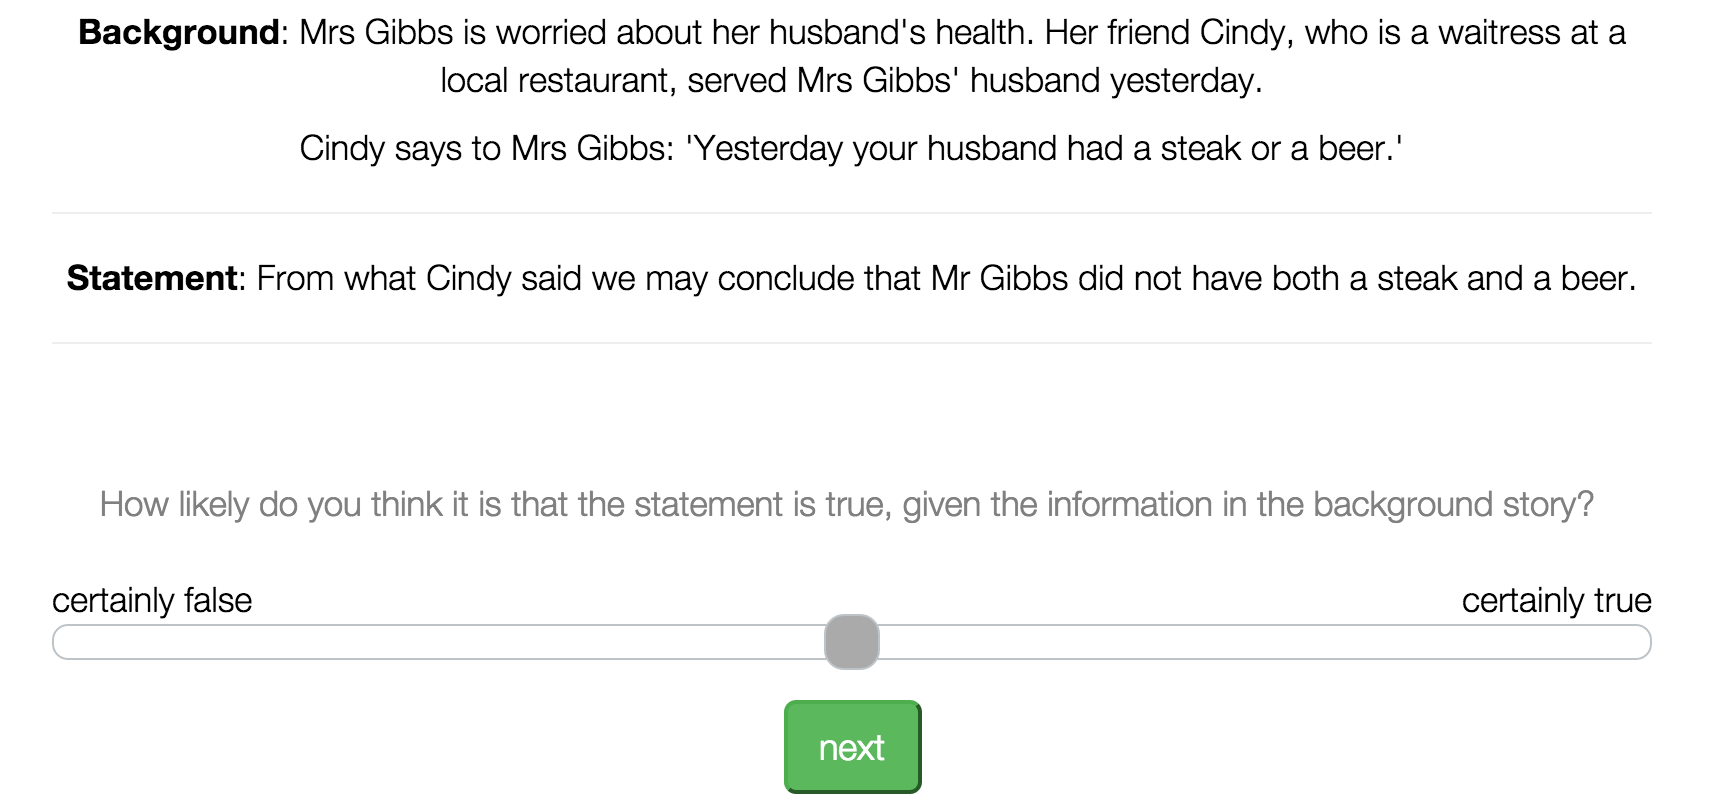
\includegraphics[width = 0.9\textwidth]{pics/expExampleShot.png}
  \caption{Example of a trial \mf{insert pic with example from main text}}
  \label{fig:exampleShot}
\end{figure}

%--------------------------------------------------------
\subsection{Data preparation} 
%--------------------------------------------------------

We coded the slider-ratings as real numbers ranging from 0
(``certainly false'') to 1 (``certainly true''). Ratings for the two conditional statements in the prior condition of Exp.\ 2 were averaged.

Seven participants were excluded from the analysis because they were not self-reported native speakers of English. We also removed another eleven participants for obviously deviant answers (e.g., blindly alternating between maximal agreement and maximal disagreement).\footnote{The
  formal criterion for exclusion was having a \emph{deviance score} greater than a fixed
  threshold, where the deviance score of a participant is the sum of the absolute differences
  between the expected answers for all control questions (0, 0.5, or 1) and the subjects'
  answers. % The mean deviance score was 1.758; its standard deviation is 0.862.
  We set the threshold of exclusion to the mean plus twice the standard deviation. This
  exclusion criterion was also used in all other experiments.}  Consequently, data from a total
of 193 (Exp.\ 1) and 192 (Exp.\ 2) participants made it into our analysis. Unfortunately, there
was a mistake in the formulation of two stories, one for each experiment. We removed all data for these stories for the analysis. (See Appendix A.)

In what follows, we discuss the results of Exps.\ 1 and 2 in turn, starting with Exp.\ 1, which tested the upper-bounded construal of `some'.

%--------------------------------------------------------
\subsection*{Experiment 1: Results}
%--------------------------------------------------------

\paragraph{Controls.} Ratings for control statements are unsurprising. Means, averaged over all
vignettes, for ratings of false (0.22), uncertain (0.39) and true statements (0.80) are
pairwise different (two-population directed $t$-test: $t \approx - 3.83, p < 0.001$ for false
vs.~uncertain; $t \approx - 9.98, p < 0.001$ for uncertain vs.~true).

\paragraph{Explanatory factors.} Statements that targeted relevance, competence and prior
probability were rated in accordance with our intuitive classification (see
Figure~\ref{fig:factorBoxPlotsExp3}, all high/low constrasts are significantly different).

\begin{figure}
  \centering

  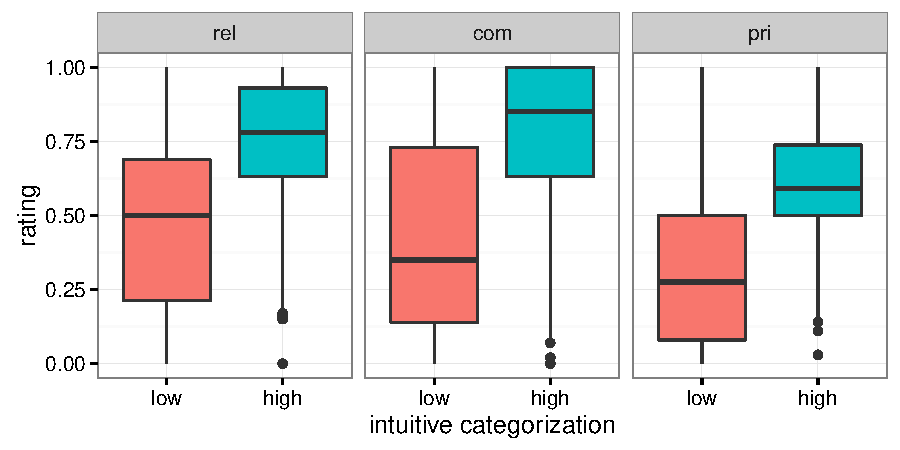
\includegraphics[width = 0.9\textwidth]{pics/factorBoxPlotExp3.pdf}
  
  \caption{Ratings of statements according to intuitive pre-classification in Experiment~1}
  \label{fig:factorBoxPlotsExp3}
\end{figure}

Figure~\ref{fig:correlationsExp3} shows the relation of per-vignette mean implicature ratings
and per-vignette mean ratings for the three explanatory factors. From visual inspection, it
seems that \rel and \com are unlikely good predictors of implicature strength, while low values
of \pri seem to be correlated with high implicature ratings, as expected.

\begin{figure}
  \centering

  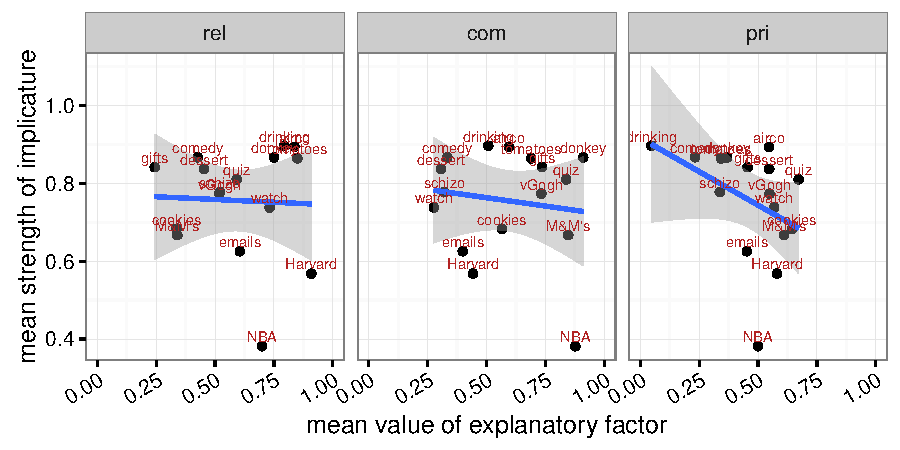
\includegraphics[width = 0.9\textwidth]{pics/correlationExp3.pdf}
  
  \caption{Per-vignette means of ratings of relevance, competence and prior statements
    vs. per-vignette means of implicature rating in Experiment~3}
  \label{fig:correlationsExp3}
\end{figure}

\paragraph{Main analysis.} We want to explain ratings of the \emph{Inference}-statement in
terms of explanatory factors \rel, \pri, and \com, which are the respective means of ratings of
the corresponding statements for each vignette. Figure~\ref{fig:BFsExp3} gives the Bayes
factors of regression models with our three explanatory variables as main factors. The best
model only contains factor \pri and is made roughly six times more likely by the data than the
two runner-ups which contain additionally \rel or \com. Clearly, the data provides very strong
evidence in favor of all models that include \pri, relative to those which do not.

\begin{figure}
  \centering
  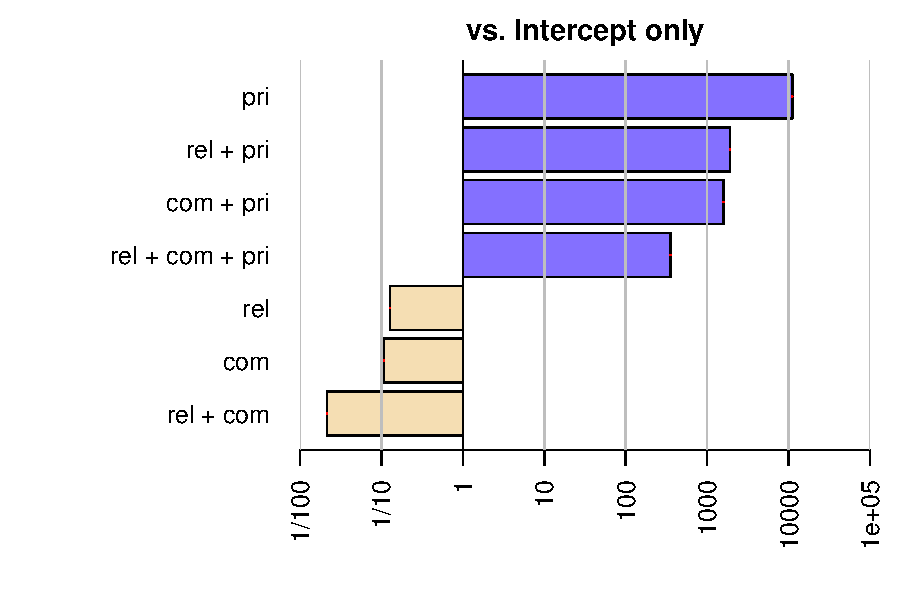
\includegraphics[width = 0.8 \textwidth]{pics/bfsAllExp3.pdf}
  \caption{Bayes factor comparison of different main factor combinations, predicting the
    strength of scalar enrichment of \emph{some} in Experiment~1.}
  \label{fig:BFsExp3}
\end{figure}

\paragraph{Controls in Exp.\ 2.} Control statements were rated as expected, indicating that participants
understood the task in general and paid attention to the background stories. Means, averaged
over all vignettes, for ratings of false (0.26), uncertain (0.48) and true statements (0.81)
are pairwise different (two-population directed $t$-test: $t \approx - 3.72, p < 0.001$ for
false vs.~uncertain; $t \approx - 6.93, p < 0.001$ for uncertain vs.~true).

% Figure~\ref{fig:densityFactors} shows estimated density estimates of the ratings given to the
% four factors of interest, averaged over all vignettes. Competence ratings tend towards full
% uncertainty (mean $\approx 0.51$, standard deviation $\approx 0.34$), similarly for relevance
% ratings (mean $\approx 0.53$, standard deviation $\approx 0.3$). Prior ratings were generally
% lower (mean $\approx 0.37$, standard deviation $\approx 0.25$), and ratings for the disjunctive
% statement higher (mean $\approx 0.63$, standard deviation $\approx 0.33$).

% \begin{figure}[t]
%   \centering

%   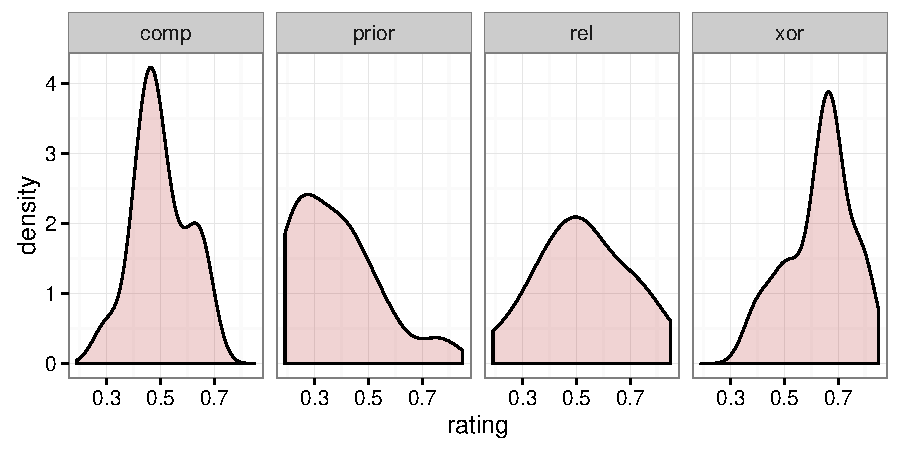
\includegraphics[width = 0.9\textwidth]{pics/densityFactorsExp1.pdf}
  
%   \caption{Density estimates for distribution of ratings across all vignettes}
%   \label{fig:densityFactors}
% \end{figure}

\paragraph{Explanatory factors.} Ratings of relevant explanatory factors are not uniformly
distributed across vignettes, but validate our intuitive pre-classification (see
Figure~\ref{fig:factorBoxPlots}, all high/low contrasts are significant).

\begin{figure}[t]
  \centering

  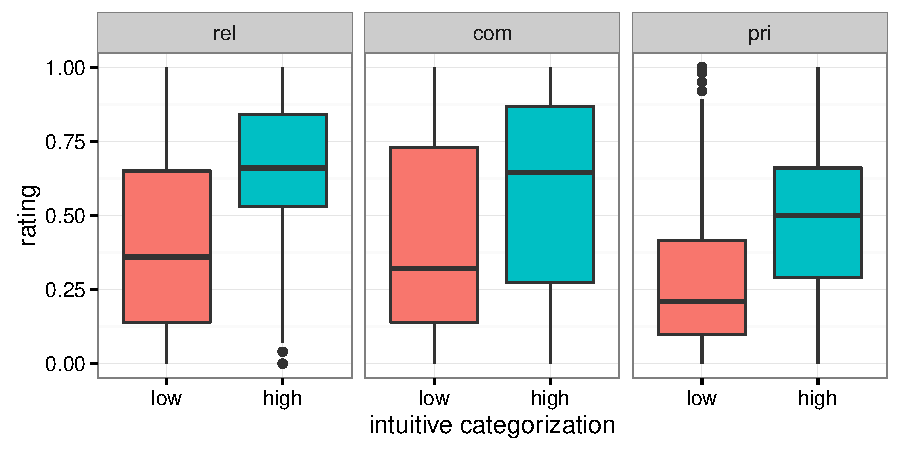
\includegraphics[width = 0.9\textwidth]{pics/factorBoxPlotExp1.pdf}
  
  \caption{Ratings of statements according to intuitive pre-classification in Experiment~1}
  \label{fig:factorBoxPlots}
\end{figure}

Figure~\ref{fig:correlationsExp1} shows the relation of per-vignette mean implicature ratings
and per-vignette mean ratings for the three explanatory factors. From visual inspection, it
seems that relevance and competence are not good predictors of implicature strength, while low prior
plausibility seems to be correlated with high implicature ratings, as expected.

\begin{figure}[t]
  \centering

  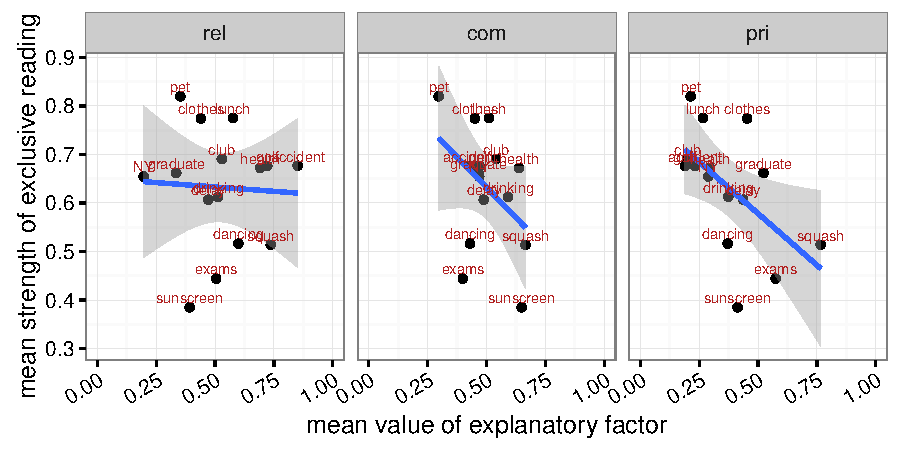
\includegraphics[width = 0.9\textwidth]{pics/correlationExp1.pdf}
  
  \caption{Per-vignette means of ratings of relevance, competence and prior statements
    vs. per-vignette means of implicature rating in Experiment~1}
  \label{fig:correlationsExp1}
\end{figure}

\paragraph{Main analysis.} To check whether factors ``relevance,'' ``prior'' and ``competence''
have an influence on the strength of exclusive readings, we compare regression models of
different complexity. The dependent variable are ratings of the
\emph{Xor}-statement. Explanatory factors \rel, \com, and \pri are, respectively, the means of
the ratings, for each vignette, of the \emph{Relevance}, \emph{Competence} and \emph{Prior}
statements. We take a Bayesian approach to comparing regression models in terms of their Bayes
factors \citep{RouderMorey2012:Default-Bayes-F}, as implemented in the \emph{BayesFactor}
$R$-package. This gives us a more nuanced picture of the relative evidence for models of
different complexity, including information about how much, e.g., the absence of a factor in a
model, is supported by our data.\footnote{All conclusions of theoretical relevance are also
  supported by more traditional, frequentist regression analyses in terms of significance of
  factors and model comparison by AIC.}

\begin{figure}
  \centering
  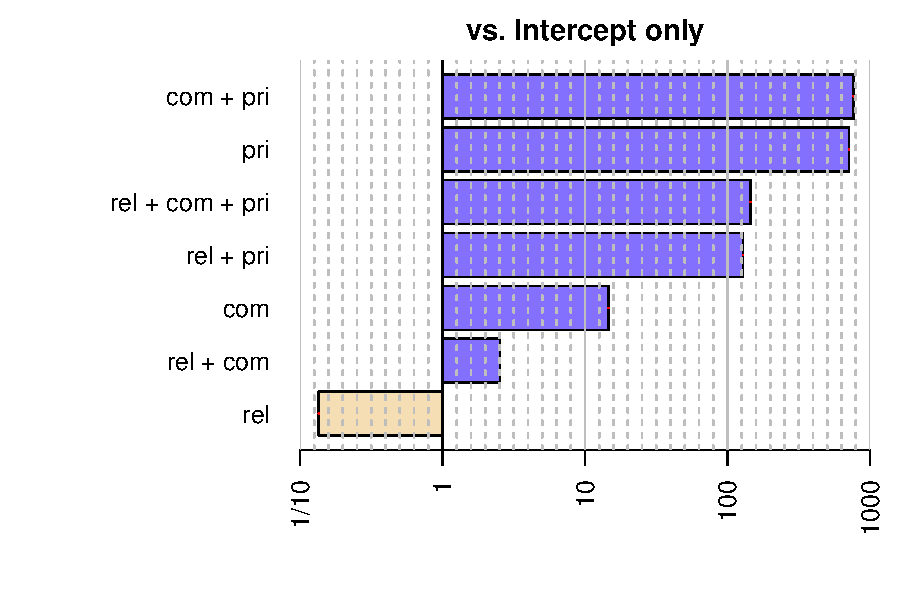
\includegraphics[width = 0.8 \textwidth]{pics/bfsAllExp1.pdf}
  \caption{Bayes factor comparison of different main factor combinations. Notation like ``com +
    pri'' stands for a regression model with main factors \com and \pri.}
  \label{fig:BFs}
\end{figure}


Figure~\ref{fig:BFs} shows the Bayes factors of all regression models that can be built with
our three explanatory variables as main factors. The graph gives the Bayes factor of each
regression model, listed on the right, against the intercept-only model. A model with only \rel
as a main factor, for example, is roughly 8 times worse than the intercept-only model,
suggesting that \rel alone makes no useful contribution to harnessing the variance in
\emph{Xor}-ratings, but only makes for a more complex model. Single main factor \com does make
a significant contribution, compared to the intercept-only model, but a model with single main
factor \pri is more than 30 times more likely, given our data, than the model with just
\com. The best model, by this standard, is a model with \com and \pri as main effects, but
there is no substantial difference between this and the model with only \pri as a main factor.

The main conclusion to be drawn from this analysis is that \rel is a bad, \com an unnecessary,
and \pri the best predictor of strength of exclusive readings.\footnote{This general conclusion
  is also vindicated by more complex analyses that would take interactions and random effects
  for participants into account.} Factor \rel should be omitted for reasons of parsimony (every
model with it is worse than the corresponding one with it), while \com can be omitted at no
substantial loss (adding \com makes models better, but not substantially so, when \pri is
present). Omitting \pri leads to a substantial decline in explanatory power.

Estimates of the posterior distributions over model parameter coefficients for the linear model
that contains all three factors \rel, \com and \pri are shown in
Figure~\ref{fig:densityMCMC}. Noteworthily, most credible values for coefficients for \com are
negative. This is the same for all other models containing factor \com. This means that our
data suggests that the more competent the speaker was felt to be, the lower the strength of the
exclusive reading. This is the reverse of what we would expect from basically all pragmatic
theories. In contrast, the impact of \pri is as expected: the more likely the conjunctive
alternative, the less strong the exclusive reading is felt to be.

\begin{figure}
  \centering
  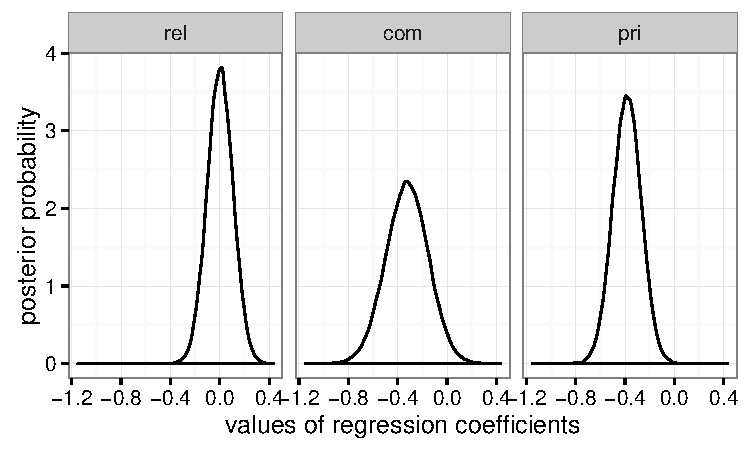
\includegraphics[width=0.8\textwidth]{pics/densityMCMCExp1.pdf}
  \caption{Density estimates of posterior over model parameter coefficients for a linear model
    with all three main factors.}
  \label{fig:densityMCMC}
\end{figure}

\subsection*{Discussion.} Prior plausibility of the conjunctive alternative seems to be the
main explanatory factor of \emph{Xor}-ratings. This is interesting since standard theories
usually do not emphasize the role of prior plausibility. Moreover, it is actually surprising
from the point of view of standard pragmatic theories of exclusive disjunction readings that
relevance does not seem to play an explanatory role and that competence is correlated with
\emph{Xor}-strength in the ``wrong direction,'' so to speak. \mf{more here? or rather later?}

Before drawing firm conclusions, we should address some potential worries about this design and
the evidence that our results provide for or against theoretical positions. First of all, it
could be objected that the way in which we measured factor \pri is inadequate. What matters, so
a possible objection goes, is the prior plausibility of ``$A$ and $B$'' not the mean of the
plausibility of conditionals ``if $A$, $B$'' and ``if $B$, $A$.'' Experiment~2 presents a
follow-up that addresses this issue. Secondly, we should verify that our experimental measures
of relevance, competence and prior do what we would like them to. In order to address this
issue, Experiment~3 looks at scalar quantifier \emph{some} in a parallel design to that of
Experiment~1.



\subsection*{Results}

\paragraph{Data preparation.} Four participants were excluded from the analysis because they
were not self-reported native English speakers. Another 6 participants were excluded for poor
performance, by the same criterion as used with Experiment~1. All data from the remaining 193
participants entered into the analysis.



\subsection{Discussion}

We could conclude from this analysis that \pri is the key factor in our regression model
comparison for predicting the strength of scalar inferences.\footnote{This is also the case for
  more complex analyses that take interactions and random effects for participants into
  account: the model with only \pri as factor is the best, and every model that contains it is
  strongly favored by the data above any model that does not.} Factors \rel and \com do not
seem to carry extra explanatory power. This would suggest that the behavior of scalar
\emph{some} parallels that of disjunction \emph{or} in terms of which factors seem to influence
the strength of the putative implicatures. 

There is, however, a particular oddity in our data. A look back at
Figure~\ref{fig:correlationsExp3} reveals that one vignette received a surprisingly low mean
score for implicature strength, namely \emph{NBA}. When we compare the ratings of the
\emph{notAll}-statement given for the \emph{NBA} vignette with those given for each other
vignette, we see that all of these fifteen pairwise comparisons shows a significant
difference. No other vignette had that property in Experiment~3, and also no vignette from
Experiment~1 was an ``outlier'' in this sense. Low implicature ratings for this vignette are
particularly surprising, because it was intuitively classified as high relevance, high
competence, and low prior. So, all explanatory factors should, by the standard theory, point
towards high implicature rates. The observed ratings of these factors for this vignette
accorded with intuition. Moreover, the NBA story had remarkably many participants answering
that the likelihood of the implicature was exactly zero. Eight participants provided such a
response; none did so for the next lowest-scoring item. Clearly, this case seems to stand out
in some way.

% One thing that is special about the \emph{NBA} vignette is that not only the speaker is
% introduced as an expert, but also the listener. This vignette is the only one, including
% vignettes from Experiment~1, in which the listener does not seek factual information from the
% speaker. It is the only vignette in which the listener is likely to know whether the
% \emph{all}-situation is true. This may lead subjects to see a different purpose in the
% utterance of the speaker than to provide useful information, if that is measured in terms of
% logical strength. The kind of information that the speaker offers in this vignette is, perhaps,
% much better construed as evidence in favor of a conclusion that is under debate
% \citep{Ducrot1973,AnscombreDucrot1983:Largumentation-,MerinInfoRelSocialDecisionmaking1999,Rooijvan-Rooij2004:Cooperative-ver}. 

% In a sense it is rather unusual that the NBA item should score so low, given how unlikely it is that any one player should score the decisive points in the dying seconds of all playoff games. Indeed, there are several observations indicating that something went wrong with this particular item. First, of course, is the extremely low implicature rating (0.39) compared to the next lowest scoring item (0.58). For comparison, the difference between the second and third lowest scoring items was less than 0.05. Second, the NBA story had remarkably many participants answering that the likelihood of the implicature was 0.00. Eight participants provided such a response; none did so for the next lowest-scoring item.

Here is what we believe went wrong with this item. Consider the \emph{notAll}-statement of this
vignette:

\begin{quote} \emph{notAll} \\
  From what Jason Barley said we may conclude that Greg Jones did not secure victory for his
  team during the last seconds of all of the decisive playoff matches.
\end{quote}

\noindent Rather than directly modifying the noun phrase, the negation modifies the verb phrase
and is separated by three constituents from the noun phrase. This may invite a reading, which
was not intended, in which the negation modifies the verb rather than the noun phrase. In other
words, it invites a reading of the complement of `said' that can be paraphrased as `Greg Jones
failed to secure victory for his team during the last seconds of all of the decisive playoff
matches.' We suspect that participants arrived at this reading because of the amount of
material between the negation and the noun phrase, which invited participants to instead have
the negation modify the verb. Indeed, we found that ratings of exactly zero were overall much
more frequent in cases of VP-negation than in cases of NP-negation. \mf{I don't understand the
  last sentence.  Where did we find that? Should we really mention this? Should we go into the
  NP- vs. VP-negation thing in more detail? Otherwise, maybe drop this?}

In order to test our hypothesis that participants arrived at an unintended reading of the
target statement, we conducted a small follow-up experiment in which we gathered implicature
ratings for a statement that better expressed the intended reading than the one used in
Experiment 3:

\begin{quote} From what Jason Barley said we may conclude that not all of the decisive playoff matches were secured during the last seconds by Greg Jones. \end{quote}

\noindent The follow-up consisted of the NBA story followed by three statements: two control
statements and one target statement. The target statement was varied between the one used in
Experiment 3 (see above) and the alternative one with NP-negation, and was varied between
participants. 40 participants were drafted on Mechanical Turk and were paid \$0.15 for their
participation. They were instructed to, first, read the story carefully and, afterwards,
indicate the likelihood of the corresponding statements on a seven-point Likert scale. We
hypothesised that implicature ratings would be substantially higher for the modified statement
than for the original one.

The normalised implicature ratings for the original statement were slightly lower than in
Experiment 3 (0.25 versus 0.39). Crucially, however, the normalised implicature ratings for the
modified statement were significantly higher and much more in line with what we observed for
the other items (0.76, $t$(29) = 4.28, $p$ $<$ .001). Since the two statements were synonymous
on their intended readings, we consider this compelling evidence that participants in
Experiment 3 arrived at an unintended reading of the target sentence and sufficient reason for
discarding the item from our analysis.

Consequently, we reran the regression model comparison after excluding all data from the
\emph{NBA} vignette. The results are shown in Figure~\ref{fig:BFsExp3noNBA}. The best model
considers only factors \com and \pri. It is more than 6 times likelier, given the data, than
the second best model, which also includes \rel, which in turn is about 3.5 times likelier than
the third model with single factor \pri. Figure~\ref{fig:BFsExp3noNBA_regressionCoefficients}
shows posteriors over regression coefficients for that model with main effects \rel, \com and
\pri. Unlike for the disjunction case in Experiment~1, the effect of factor \com on strength of
scalar enrichment is as expected from standard theory: the more competent a speaker is felt to
be, the stronger the scalar implicature reading.


\begin{figure}
  \centering
  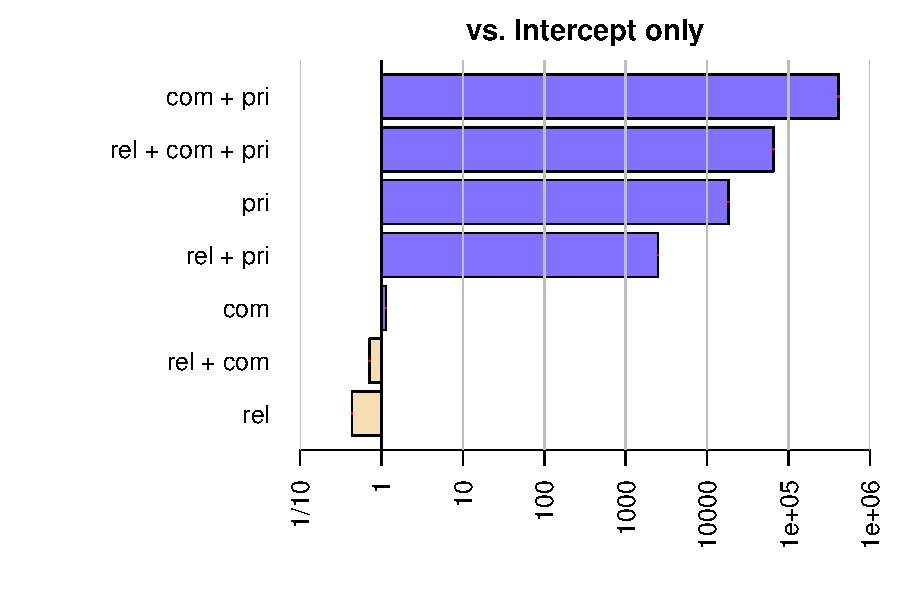
\includegraphics[width = 0.8 \textwidth]{pics/bfsAllExp3_noNBA.pdf}
  \caption{Bayes factor comparison of different main factor combinations, predicting the
    strength of scalar enrichment of \emph{some} in Experiment~3 after excluding data from the
    ``NBA'' scenario.}
  \label{fig:BFsExp3noNBA}
\end{figure}

\begin{figure}
  \centering
  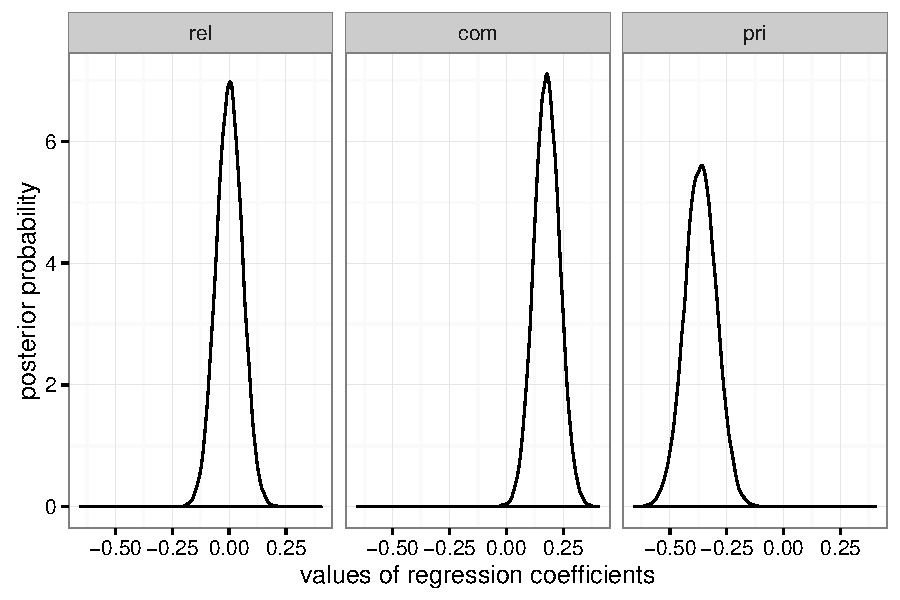
\includegraphics[width = 0.8 \textwidth]{pics/densityMCMCExp3.pdf}
  \caption{\mf{fill me}}
  \label{fig:BFsExp3noNBA_regressionCoefficients}
\end{figure}

In sum, we believe that there are good reasons to exclude the \emph{NBA} vignette from our
analysis, because of an unintended ambiguity in the \emph{notAll}-statement. Doing so, reveals
that factors \pri and \com contribute most to explaining the variance in implicature
strength. Just as for disjunction, relevance seems to be a superflous factor, because any model
without factor \rel is worse than the corresponding one where it is added. This suggests that
the speaker expertise paradox \mf{terminology?} may be a real problem. While manipulations of
competence do have the effects predicted by standard theories of scalar implicature for the
case of \emph{some}, this is not the case for disjunctive readings of \emph{or}. There does
seem to be a difference, which is, as such, already unexpected under standard conceptions.


\section{Experiment~4}

\subsection{Design}

Exclusive readings of disjunctions can also come about by exhaustifying individual disjuncts
(see Section~XYZ). This approach would predict that the strength of an exclusive disjunction
reading of ``$A$ or $B$'' should be positively correlated with the strength of exhaustive
readings that statements of individual disjuncts ``$A$'' and ``$B$'' would receive in the same
context. The purpose of Experiment~4 was therefore to collect data on the strength of
exhaustive readings of such single-disjunct statements in the background contexts used in
Experiment~1. We would then like to investigate whether strengths of exhaustive readings make
for a reliable predictor of strength of exclusive readings across contexts.

\subsection{Participants}

Using the same selection criteria as before, 131 subjects were recruited via Amazon's
Mechanical Turk and paid US\$ 0.50 for participation.

\subsection{Materials}

Experiment~4 used the fifteen vignettes from Experiment~2 (that is excluding the erroneous
``Bill's orders'' scenario). For each vignette we consider the speaker's utterance of single
disjuncts (see Appendix~\ref{sec:mater-exper-1}). Concretely, where Experiment~1 had an
utterance of a disjunction:

\begin{quote}
  \emph{Utterance of disjunction}\\
  Jill says to Danny: `Alex bought a racket or a pair of shoes.'
\end{quote}

\noindent Experiment~2 had two single-disjunct utterances by the same speaker:

\begin{quote}
  \emph{Utterance of disjunct 1}\\
  Jill says to Danny: `Alex bought a racket.' \\[.2cm]
  \emph{Utterance of disjunct 2}\\
  Jill says to Danny: `Alex bought a pair of shoes.'
\end{quote}

\noindent Additionally, each vignette also had corresponding statements that subjects had to
rate:

\begin{quote}
  \emph{Exh1}\\
  From what Alex's girlfriend said we may conclude that Alex did not buy a pair of shoes as well. \\[.2cm]
  \emph{Exh2}\\
  From what Alex's girlfriend said we may conclude that Alex did not buy a racket as well.
\end{quote}

\subsection{Procedure}

The procedure followed that of Experiment~2 very closely. After reading (slightly amended)
instructions and seeing examples for the use of the slider bar, each participant was presented
with six randomly sampled vignettes. Subjects read the background story, followed with an
utterance of disjunct 1 or 2, randomly chosen. Subjects first rated a random control question
and then rated the \emph{Exh1} or \emph{Exh2} statement, depending on which utterance was shown
to them.

\subsection{Results}

Data from one subject was discarded because English was not the self-reported native
language. Another four subjects were removed for bad performance on the control questions,
using the same criterion as before.

\begin{figure}
  \centering
  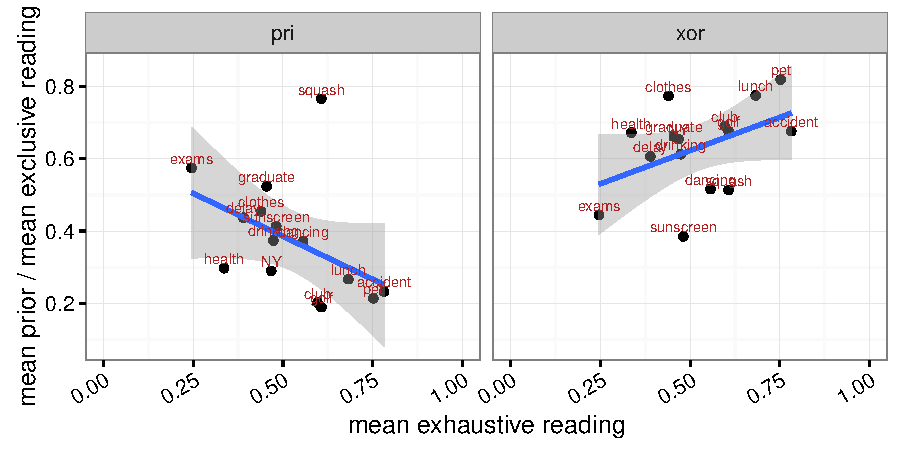
\includegraphics[width=0.9\textwidth]{pics/correlationExhXorPri.pdf}
  \caption{Means of ratings of \emph{Exh}-statements from Experiment~4 ($x$-axis) vs. means of
    ratings of \emph{Prior}-statements and \emph{Xor}-statements from
    Experiment~1 ($y$-axis)}
\label{fig:CorrelationExp1Exp4}
\end{figure}

Figure~\ref{fig:CorrelationExp1Exp4} shows the per-vignette means of the ratings of the
\emph{Exh}-statements plotted against the corresponding mean ratings of the \emph{Prior}- and
\emph{Xor}-statements from Experiment~1. There is no significant correlation between
\emph{Prior}-ratings and \emph{Exh}-ratings ($r \approx -0.44$, $p \approx 0.1$), suggesting
that our measures of prior expectations and exhaustive strength do not coincide. Adding the
per-vignette mean \emph{Exh}-ratings as an additional explanatory factor \exh to the regression
model comparison, we obtain the picture given in Figure~\ref{fig:BayesFactorsExp4}. A model
using single factor \pri to predict \emph{Xor}-ratings is about 8.5 times more likely than a
model using single factor \exh. That means that our data provides evidence for the assumption
that prior expectations are a better explanatory factor of exclusive readings than the strength
of exhaustive readings.

\begin{figure}
  \centering
  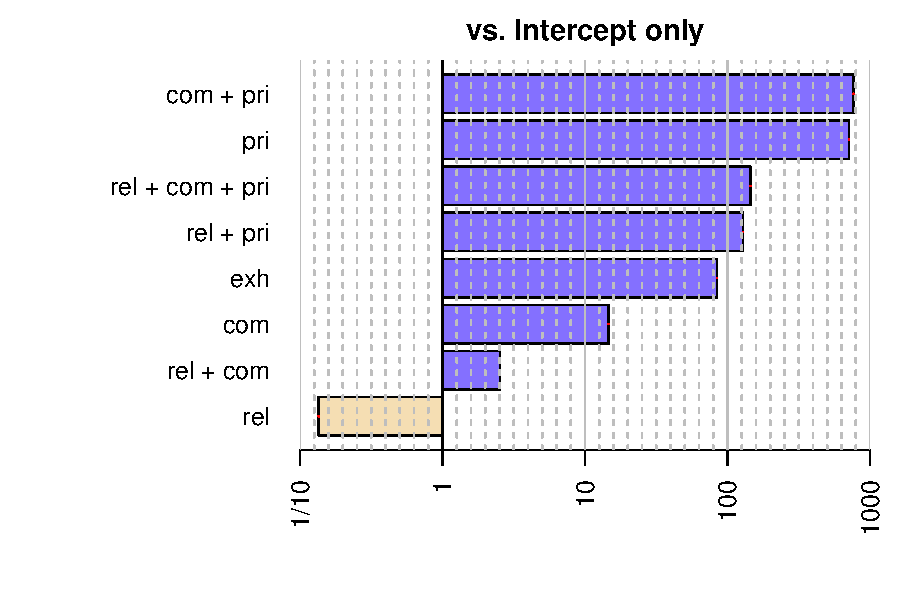
\includegraphics[width=0.9\textwidth]{pics/bfsAllExp4.pdf}
  \caption{Bayes factor comparison of different main factor combinations, predicting the
    strength of exclusive disjunction readings with additional factor \exh from Experiment~4.}
\label{fig:BayesFactorsExp4}
\end{figure}

%------------------------------------------
\section{General discussion}
%------------------------------------------

Statements of the form `$A$ or $B$' are sometimes interpreted as `$A$ or $B$ but not both'. The consensus in the recent literature is that these exclusive readings are scalar implicatures, which are inferences deriving from a pragmatic reasoning process about the speaker's intentions. A crucial assumption in this reasoning process is that the speaker is taken to be knowledgeable about whether the corresponding statement with `$A$ and $B$' is true. In this paper, we have presented data that challenge the implicature account. In contrast with the predictions made by this account, the robustness of the exclusive reading does not increase with the competence of the speaker about `$A$ and $B$'. Instead, we observed the reverse effect.

We also tested an alternative proposal, according to which the exclusive reading is derived as a scalar implicature by exhaustifying the individual disjuncts. According to this proposal, a sentence of the form `$A$ or $B$' is read, in effect, as `$A$ and nothing else or $B$ and nothing else'. This proposal predicts that the robustness of the exclusive reading depends on the robustness of the inference from $A$ to `$A$ and nothing else'. Although we did find a significant effect of this factor, it was a significantly worse predictor of the robustness of the exclusive reading than the prior probability that the statement with `and' was true. 

Taken together, these findings indicate that the exclusive reading of `or' is not a scalar implicature. Instead, we propose that exclusive readings are the result of probabilistic inferences about the state of the world. In other words, the meaning of `or' is inclusive, but hearers may exclude the possibility that both disjuncts are true based on their knowledge of the world.

Such probabilistic inferences have been shown to influence various other parts of language. A case in point is quantifying expressions. In a series of experiments, Moxey and Sanford \citeyearpar{moxey1993} presented participants with statements such as:

\ex.	\a. $Q$ people found Miss Sweden attractive.
	\b. $Q$ earthquakes occurred in California in 1951.
	
$Q$ was varied between ten quantifying expressions, including `a few' and `many'. Participants were instructed to estimate, e.g., the number of people who found Miss Sweden attractive and the number of earthquakes in California in 1951, based on the information expressed in the sentences. For most quantifying expressions, Moxey and Sanford observed that these estimates increased as a function of the prior probability. For example, the estimates would be higher for \Last[a] than \Last[b], since the prior probability that someone finds Miss Sweden attractive is higher than the prior probability that an earthquake occurs in California (see also \citealt{pepper1974}).

In a similar vein, the interpretation of gradable adjectives, such as `big' and `small', varies depending on our world knowledge. Kamp and Partee \citeyearpar{kamp1995} discuss the following minimal pair:

\ex.	\a. My two-year old son built a really tall snowman yesterday.
	\b. The D.U. fraternity brothers built a really tall snowman yesterday.
	
It is obvious that one's prior expectations about the size of the snowman are lower in the case of \Last[a] than in the case of \Last[b], thus demonstrating that the interpretation of `tall' varies depending on one's prior expections.

World knowledge and prior expectations thus influence the interpretation of various aspects of natural language. We propose that the interpretation of `or' is one such aspect:\ although, strictly speaking, a statement of the form `$A$ or $B$' leaves open the possibility that both $A$ and $B$ are true, prior expectations can modulate the likelihood of this possibility

We compared `or' with `some', which is often interpreted as `some but not all'. This upper-bounding construal is an uncontroversial example of a scalar implicature. Unlike the exclusive reading of `or', the robustness of the upper-bounding construal of `some' increased with the competence of the speaker about the truth of the corresponding statement with `and', in line with the results of Goodman and Stuhlm\"{u}ller \citeyearpar{goodman2013}. 

In addition, we observed a significant effect of prior probability:\ the robustness of the upper-bounding construal decreased with the prior probability that the statement with `all' was true. This effect ties in with recent experimental work from \citet{degen2015}, but speaks against observations made by \citet{geurts2010}. Geurts discusses examples such as the following to show that the decision to derive a scalar implicature is made independently from the prior probability that the statement with `all' is true.

\ex.	Cleo threw all her marbles in the swimming pool. Some of them sank to the bottom.

Here, according to Geurts' intuitions, the speaker communicates that some but not all of the marbles sank to the bottom, even though such a situation has an extremely low prior probability.

However, the tension between these two sets of observations may be more apparent than real. Our experiments, as well as the experiments of Degen and colleagues, tested the robustness of the scalar implicature, rather than whether or not a scalar implicature was derived. So it may well be the case that, even though people tend to construe `some' in \Last with an upper bound, they are less certain about this than if the statement were about, e.g., bread crumbs. 

Unlike competence and prior probability, relevance to the hearer's interest did not turn out to have any effect on the robustness of the upper-bounding construal of `some'. This is problematic to relevance theory, which predicts the robustness of an upper-bounding construal to be an increasing function of its importance to the hearer. It may suggest that relevance theory should adopt a more restricted notion of relevance in terms of discourse purposes \citep{cummins2015}.

An alternative explanation for the absence of an effect of relevance, however, is that we did not manipulate how relevant the upper-bounding construal was to the participant. According to this explanation, we failed to observe a significant effect because there were no differences in how relevant the upper-bounding readings were to the participants. Even though this alternative explanation warrants closer examination, there are several reasons to be sceptical about it. Perhaps the most prominent reason is that, strictly speaking, participants did not have any reason to derive the scalar implicature. The very fact that they do indicates, from a relevance-theoretic point of view, that they engaged with the story.

In summary, then, our results provide an insight in how various factors conspire in shaping differences in the robustness of scalar implicatures. It will be interesting to determine which other factors---e.g., typicality \citep{tiel2013}, prosodic and linguistic prominence \citep{breheny2006}, and politeness \citep{bonnefon2009}---have similar effects, and how these factors might interact. It may well be that these factors also hold the key in explaining the observation that different scalar expressions license scalar implicatures at substantially different rates \citep{tiel2016}.

%--------------------------------------------------------------
\appendix
%--------------------------------------------------------------

%--------------------------------------------------------------
\section{Stories from Experiment 1}
\label{sec:mater-exper-1}
\input{stories_exp1.txt}
%--------------------------------------------------------------

%--------------------------------------------------------------
\section{Stories from Experiment 2}
\label{sec:mater-exper-2}
\input{stories_exp2.txt}
%--------------------------------------------------------------




\normalsize
\section{Material for Experiment~3}
\label{sec:mater-exper-3}

\mf{fill me}


\bibliography{bibliography}


\end{document}
